\documentclass{beamer} 
\usepackage[UTF8,noindent]{ctexcap} %noindent表示无缩进
\usetheme{Madrid}
\usecolortheme{default}

\usefonttheme{professionalfonts}
\usepackage{hyperref} 
\usepackage{graphicx}
\usepackage{caption}
\usepackage{subfigure}
\usepackage{arev}
\title {DSP实验一}
\subtitle {有限长序列、频谱、DFT 的性质}
\author {展示人: }
\institute {信电学院} % 我在模版里写作 \institute[机构缩写]{邮箱}
\date {2021/10/18}
%\logo{
\includegraphics[scale = 0.05]{../logo/logo_blue.png}}




\begin{document}
%首页           
\begin{frame}
    \titlepage
\end{frame}
%目录页
\begin{frame}{目录}
    \tableofcontents
\end{frame}

\section{实验内容}
\begin{frame}{实验内容}
    \begin{block}{实验步骤} 
        \begin{enumerate}
            \item 生成五种共9个序列
            \item 绘制出每一个序列的实部、虚部、模、相角
            \item 计算每一个序列的幅度谱、频谱实部、频谱虚部
            \item 观察同种序列取不同参数时的频谱,发现它们的差异
        \end{enumerate}
    \end{block}

    \hspace*{\fill} 
    
    \begin{alertblock}{}
        步骤三中的频谱指的是该序列DFT变换之后的结果
    \end{alertblock}
    
\end{frame}

\section{代码演示}
\begin{frame}{代码演示}
   \begin{block}{代码结构}
    在本次的实验中,我将整个实验作为一个整体进行
    考虑,在Problem1.m脚本文件中调用生成各种序列以及
    绘制各种图像的函数。
   \end{block}
   \begin{block}{}
    同时将其分为三节,第一节生成9个序列,
    第二节绘制各个序列时域上的实部、虚部、幅值以及相位,第三节
    则绘制各个序列频域上的图像
   \end{block}
   \hspace*{\fill} 
   \begin{alertblock}{}
    \centering
       接下来将具体讲解各个代码
   \end{alertblock}
\end{frame}

\section{结果分析}
\begin{frame}{$x(n) = a^n$:a=0.5,length=10}
    \begin{figure}[H]
        \centering
        \begin{minipage}[t]{0.48\textwidth}
        \centering
        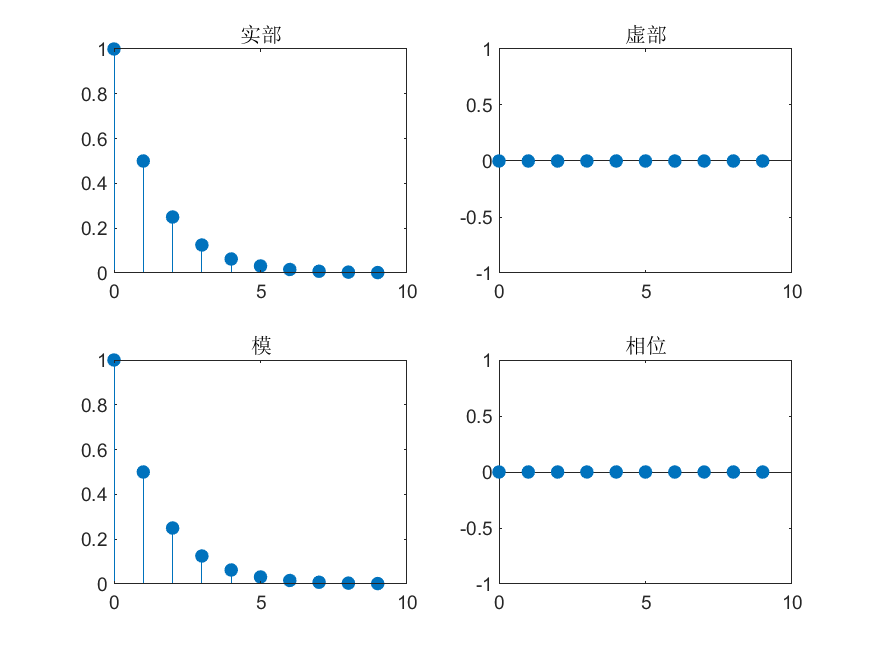
\includegraphics[width=\textwidth]{figure/实指数序列_a=05,length=10.png}
        \end{minipage}
        \begin{minipage}[t]{0.48\textwidth}
        \centering
        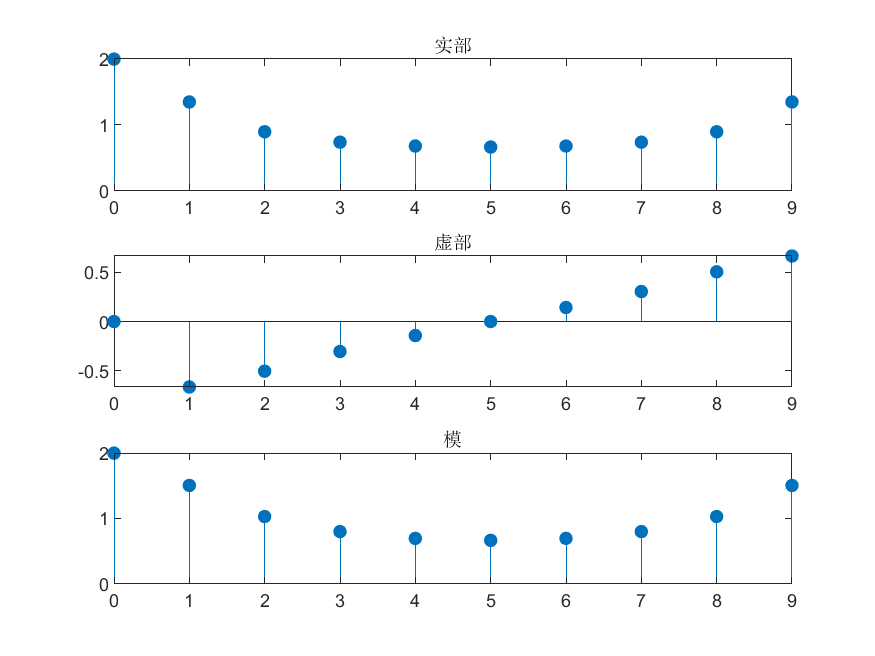
\includegraphics[width=\textwidth]{figure/频谱_实指数序列_a=05,length=10.png}
        \end{minipage}
    \end{figure}
    \begin{block}{}
        观察时域图像,因为为实指数序列,所以虚部和相位均为0;观察频域图像,可以发现他们的实部偶对称,虚部奇对称
    \end{block}
\end{frame}

\begin{frame}{$x(n) = a^n$:a=0.9,length=10}
    \begin{figure}[H]
        \centering
        \begin{minipage}[t]{0.48\textwidth}
        \centering
        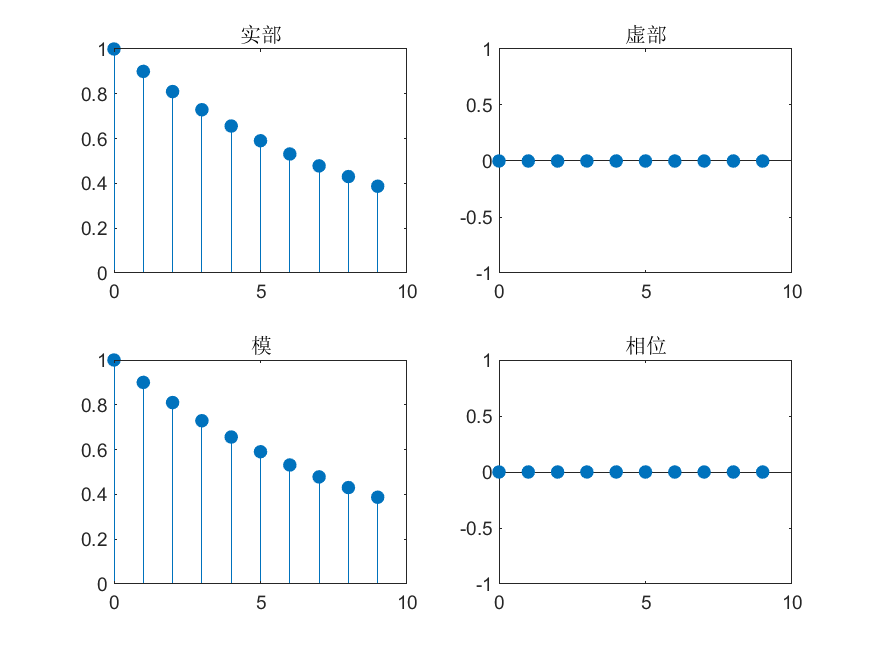
\includegraphics[width=\textwidth]{figure/实指数序列_a=09,length=10.png}
        \end{minipage}
        \begin{minipage}[t]{0.48\textwidth}
        \centering
        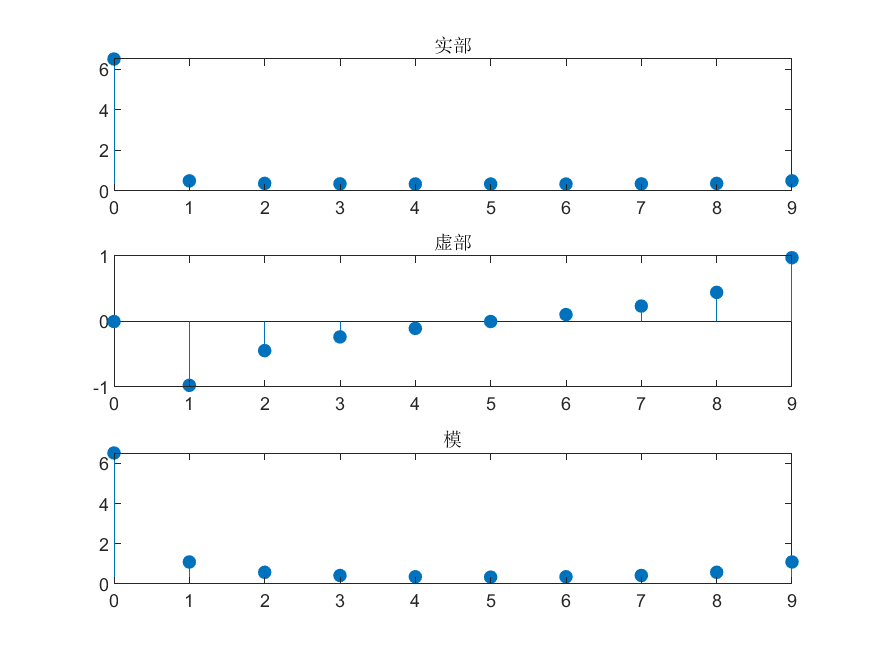
\includegraphics[width=\textwidth]{figure/频谱_实指数序列_a=09,length=10.png}
        \end{minipage}
    \end{figure}
    \begin{block}{}
        同时,我们可以发现:当a的值变大时,时域实部衰减越慢,频域X(0)的值也更大。
    \end{block}
\end{frame}

\begin{frame}{$x(n) = a^n$:a=0.9,length=20}
    \begin{figure}[H]
        \centering
        \begin{minipage}[t]{0.48\textwidth}
        \centering
        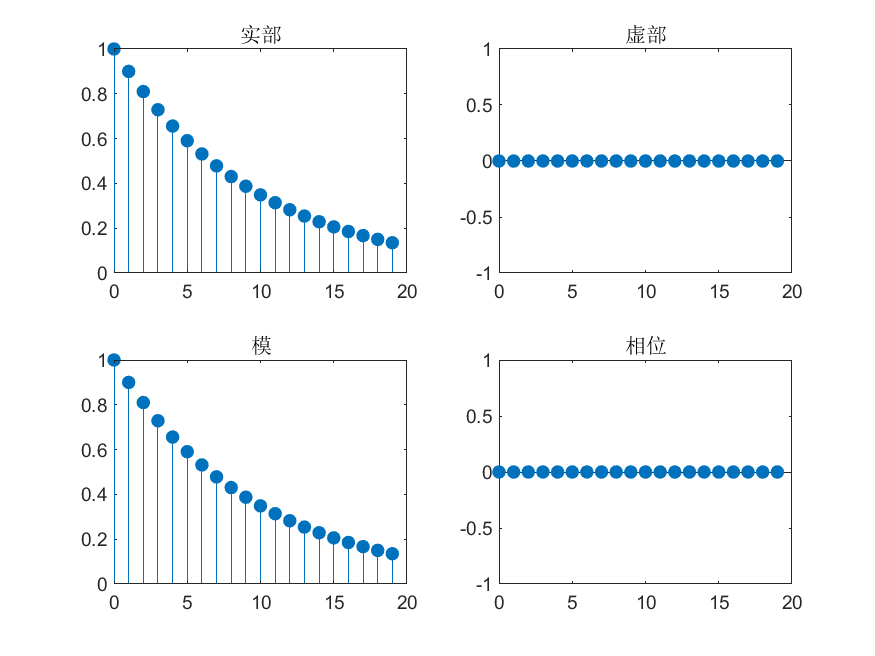
\includegraphics[width=\textwidth]{figure/实指数序列_a=09,length=20.png}
        \end{minipage}
        \begin{minipage}[t]{0.48\textwidth}
        \centering
        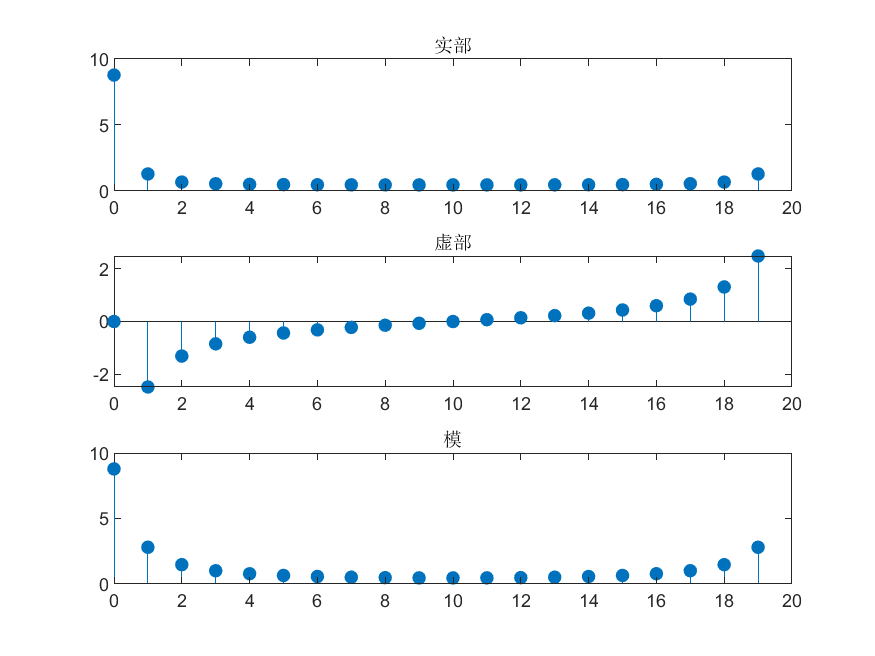
\includegraphics[width=\textwidth]{figure/频谱_实指数序列_a=09,length=20.png}
        \end{minipage}
    \end{figure}
    \begin{block}{}
        除此之外,我们也可以发现 length 越大,频谱就越接近真实图像,
这是由于采样率的提升
    \end{block}
\end{frame}

\begin{frame}[t]{复指数序列}
    \small
    \begin{figure}[H]
        \centering
        \begin{minipage}[t]{0.48\textwidth}
        \centering
        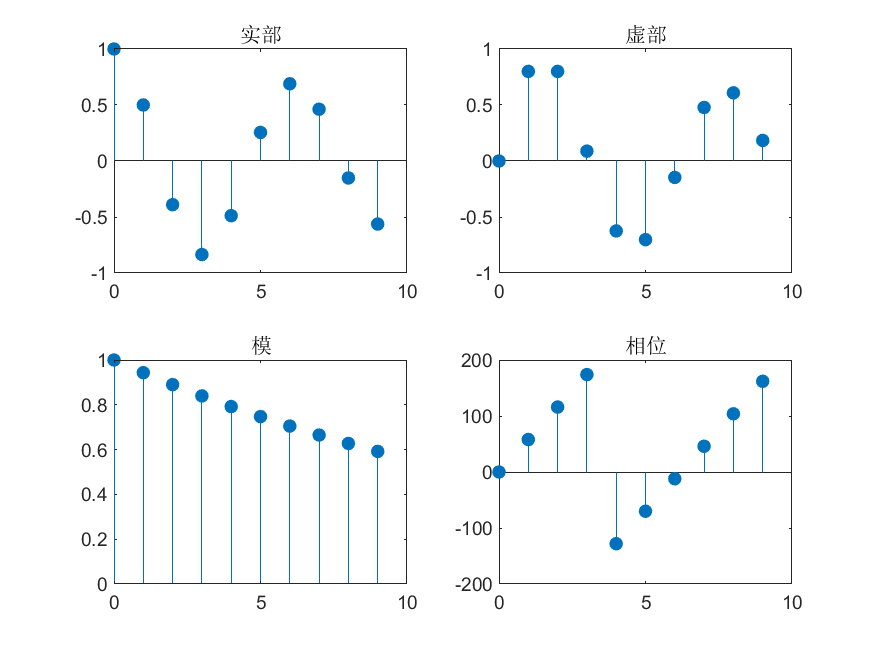
\includegraphics[width=\textwidth]{figure/复指数序列.png}
        \end{minipage}
        \begin{minipage}[t]{0.48\textwidth}
        \centering
        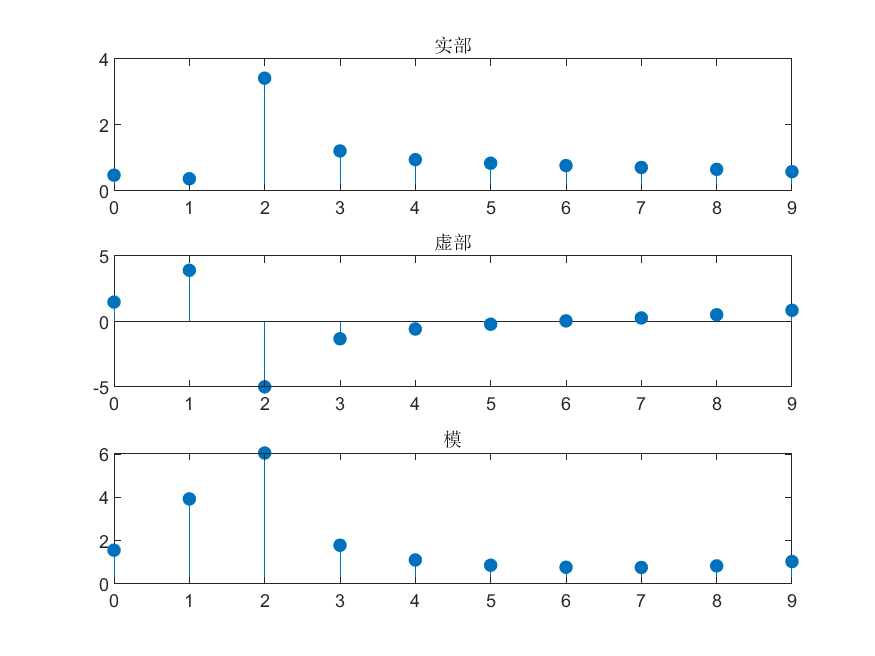
\includegraphics[width=\textwidth]{figure/频谱_复指数序列.png}
        \end{minipage}
    \end{figure}
    \begin{block}{}
        该序列为复指数序列,其可表示为$$\sqrt{a^2+b^2}e^{jn\theta} =\sqrt{a^2+b^2}(cos(n\theta)+j\sin(n\theta))$$的形式,所以时域的实部与虚部表现为正弦函数的抽样结果,相位呈现线性,因为$\sqrt{a^2+b^2}<1$,所以模减小。频域上未发现明显特点。
    \end{block}
\end{frame}

\begin{frame}[t]{正弦序列图像}
    \begin{figure}[H]
        \centering
        \begin{minipage}[t]{0.48\textwidth}
        \centering
        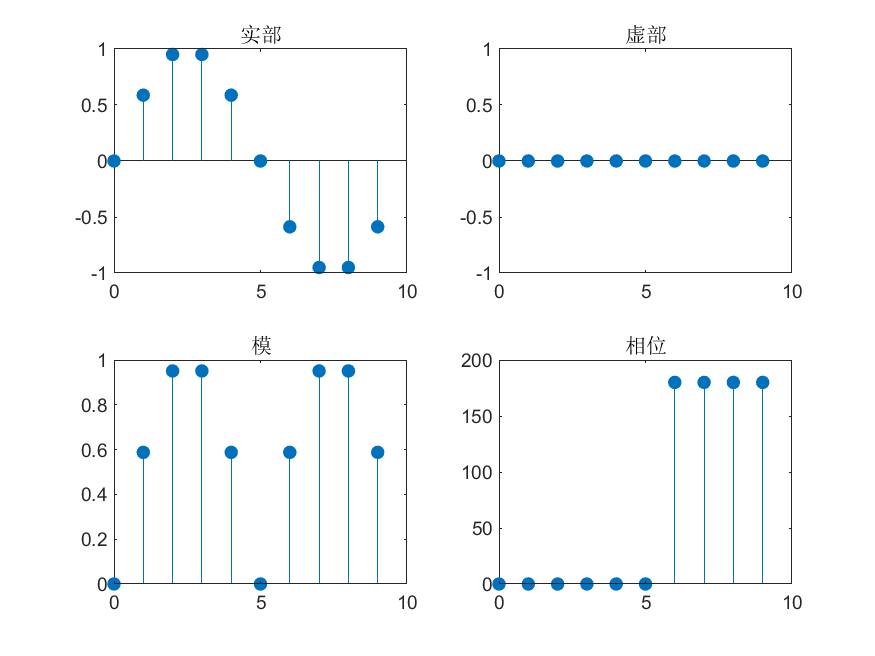
\includegraphics[width=\textwidth]{figure/正弦序列.png}
        \end{minipage}
        \begin{minipage}[t]{0.48\textwidth}
        \centering
        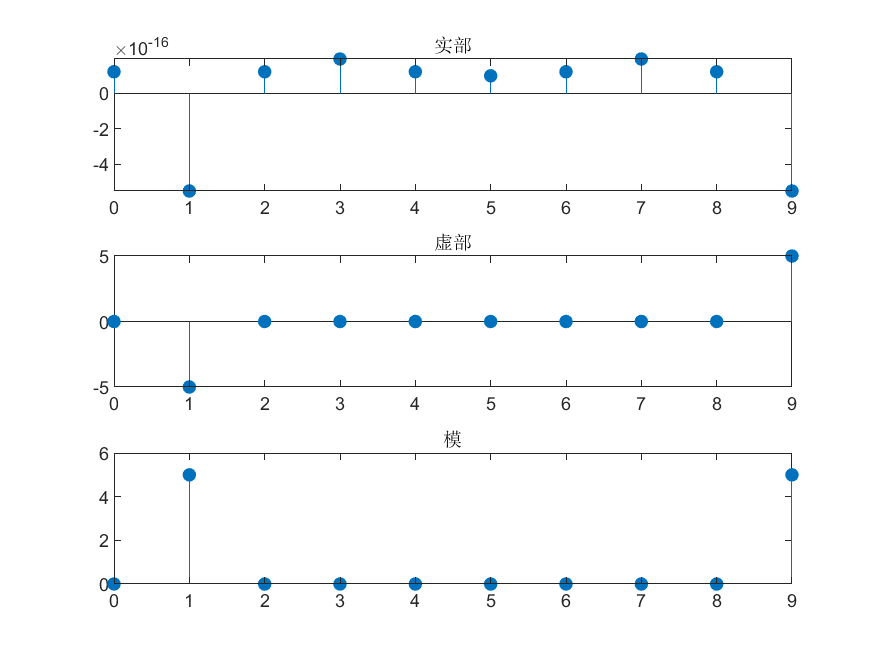
\includegraphics[width=\textwidth]{figure/频谱_正弦序列.png}
        \end{minipage}
    \end{figure}
    \begin{block}{}
        该序列是正弦函数的采样,采样周期为0.1s。观察时域图像可知:该序列为奇对称的实序列,在
x(n)大于零时相位为0,小于零时相位为 $180^\circ$。
因为该序列的对称性,所以频谱的实部应该为0,且虚部奇对称。虚部值出现在 1Hz 处,与原序列
频率吻合
    \end{block}
\end{frame}

\begin{frame}[t]{余弦序列}
    \begin{figure}[H]
        \centering
        \begin{minipage}[t]{0.48\textwidth}
        \centering
        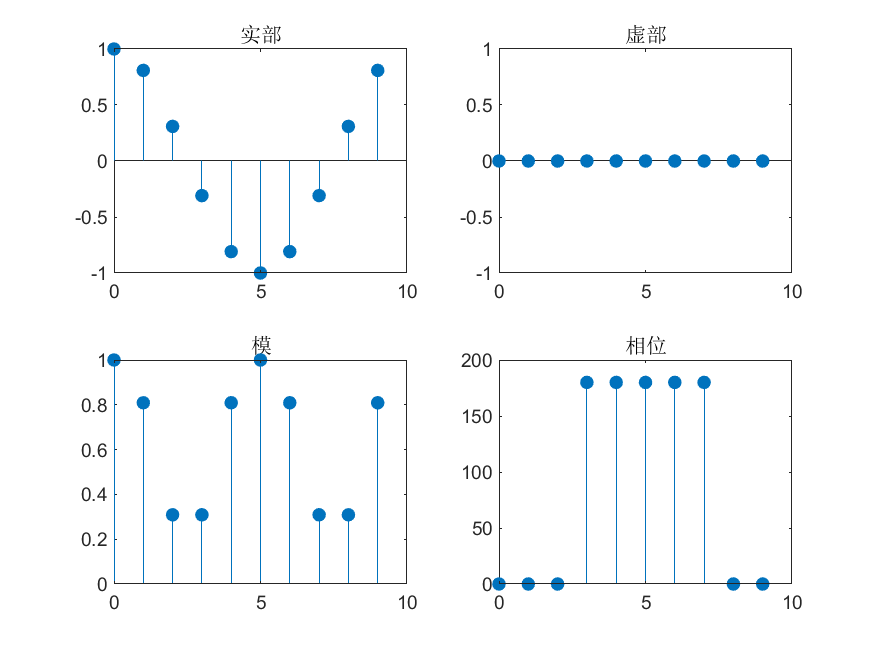
\includegraphics[width=\textwidth]{figure/余弦序列.png}
        \end{minipage}
        \begin{minipage}[t]{0.48\textwidth}
        \centering
        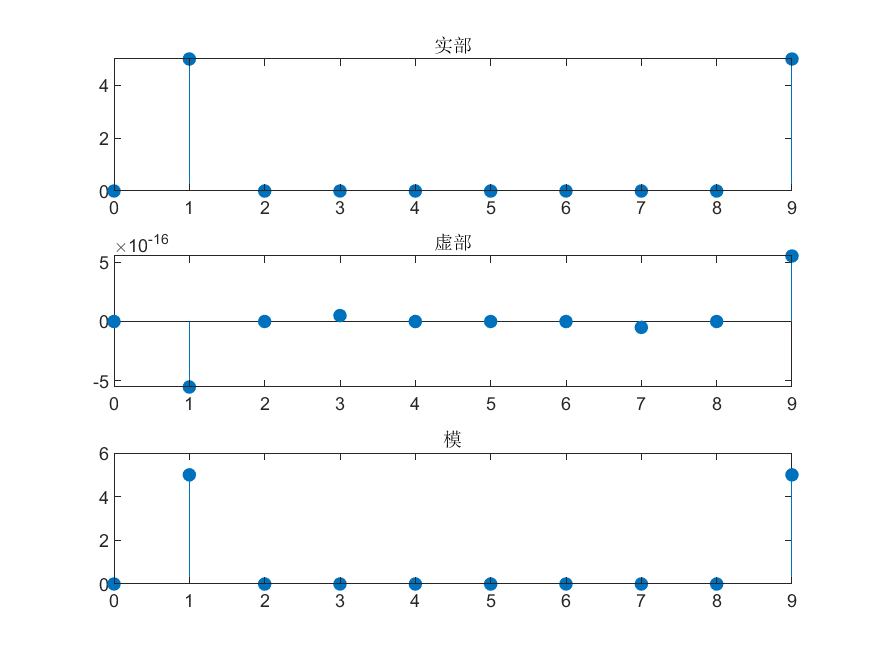
\includegraphics[width=\textwidth]{figure/频谱_余弦序列.png}
        \end{minipage}
    \end{figure}

    \begin{block}{}
        观察时域,可得该序列是偶对称的实序列,虚部为 0,相位与正弦函数类似。因为它的对称性,频
域的虚部理论上应该为 0,此处不为零是由于 MATLAB 是浮点数计算,有一定的误差,可以看出虚部
的值是一个极小的值。谱线出现在 1Hz 处,与原序列的频率吻合
    \end{block}
\end{frame}

\begin{frame}[t]{复合函数序列:$\phi = 0^\circ$}
    \begin{figure}
        \centering
        \begin{minipage}[t]{0.48\textwidth}
        \centering
        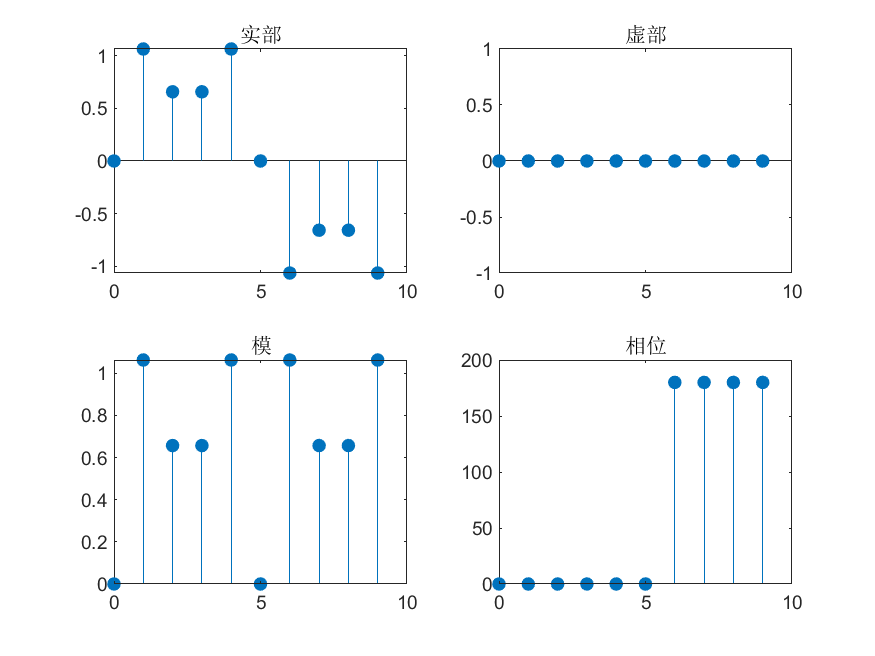
\includegraphics[width=\textwidth]{figure/复合函数序列_phi=0.png}
        \end{minipage}
        \begin{minipage}[t]{0.48\textwidth}
        \centering
        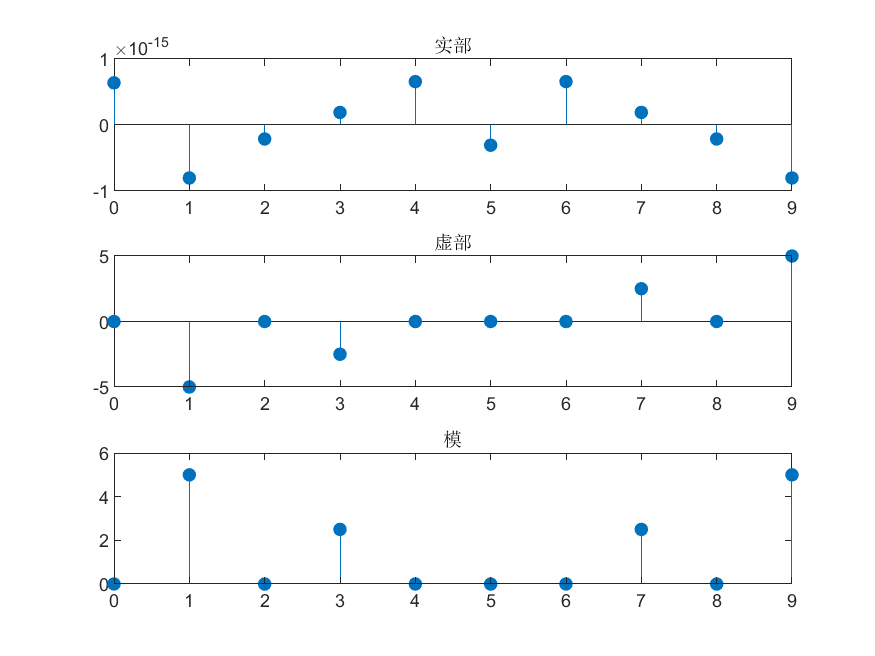
\includegraphics[width=\textwidth]{figure/频谱_复合函数序列_phi=0.png}
        \end{minipage}
    \end{figure}

    \begin{block}{}
        该序列是一个由频率为1Hz和频率为3Hz的两个序列复合而来的实序列,虚部为0. 当$\phi =0\circ | 180\circ$
时,该序列为奇序列,所以频谱实部趋近于0,虚部奇对称。因为复合的序列的频率,所以频域谱线出现在 1Hz 与 3Hz 处。
    \end{block}

\end{frame}

\begin{frame}[t]{复合函数序列:$\phi = 180^\circ$}
    \begin{figure}
        \centering
        \begin{minipage}[t]{0.48\textwidth}
        \centering
        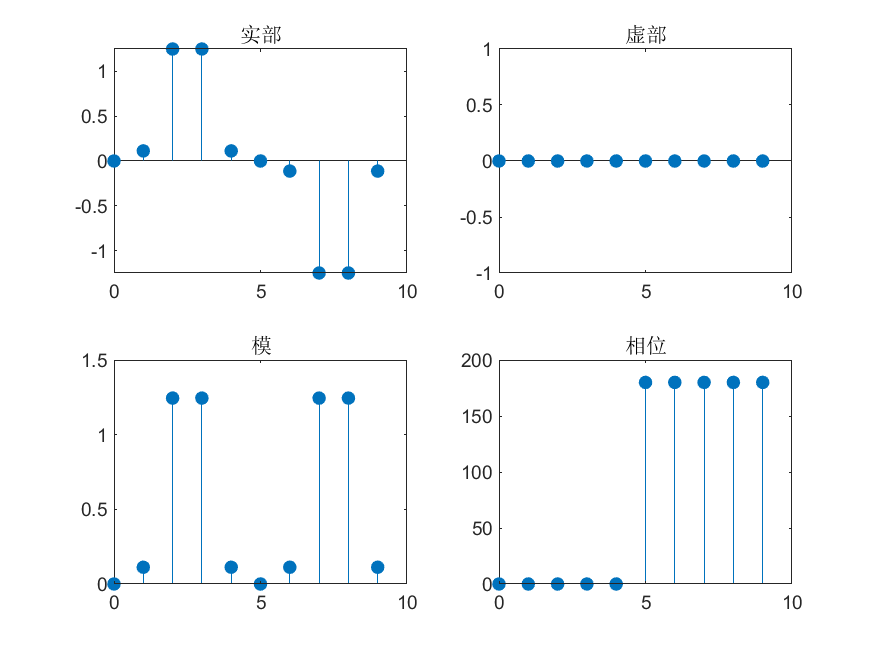
\includegraphics[width=\textwidth]{figure/复合函数序列_phi=180.png}
        \end{minipage}
        \begin{minipage}[t]{0.48\textwidth}
        \centering
        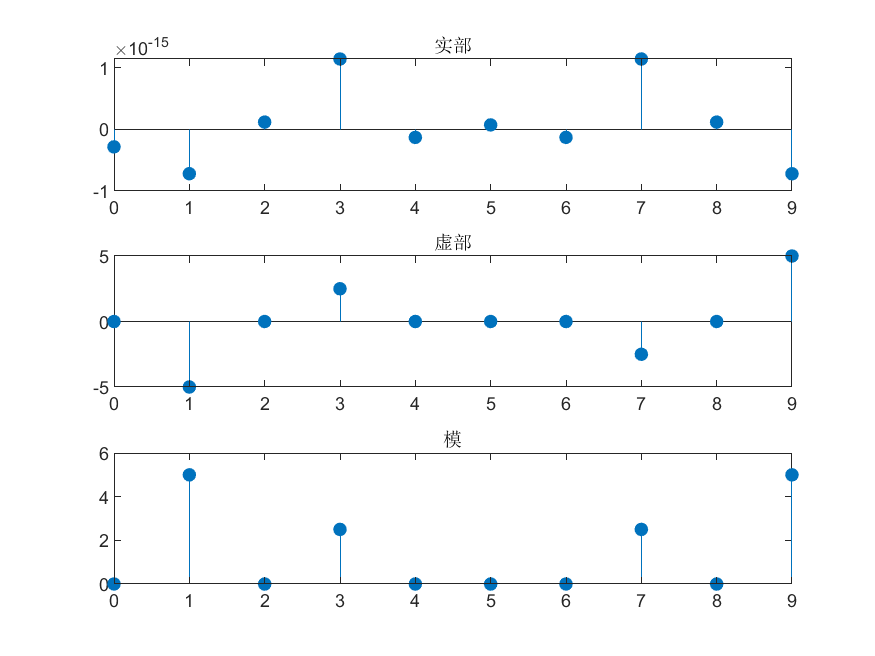
\includegraphics[width=\textwidth]{figure/频谱_复合函数序列_phi=180.png}
        \end{minipage}
    \end{figure}

    \begin{block}{}
        该序列是一个由频率为1Hz和频率为3Hz的两个序列复合而来的实序列,虚部为0. 当$\phi =0^\circ | 180^\circ$
时,该序列为奇序列,所以频谱实部趋近于0,虚部奇对称。因为复合的序列的频率,所以频域谱线出现在 1Hz 与 3Hz 处。
    \end{block}

\end{frame}

\begin{frame}[t]{复合函数序列:$\phi = 90^\circ$}
    \begin{figure}
        \centering
        \begin{minipage}[t]{0.48\textwidth}
        \centering
        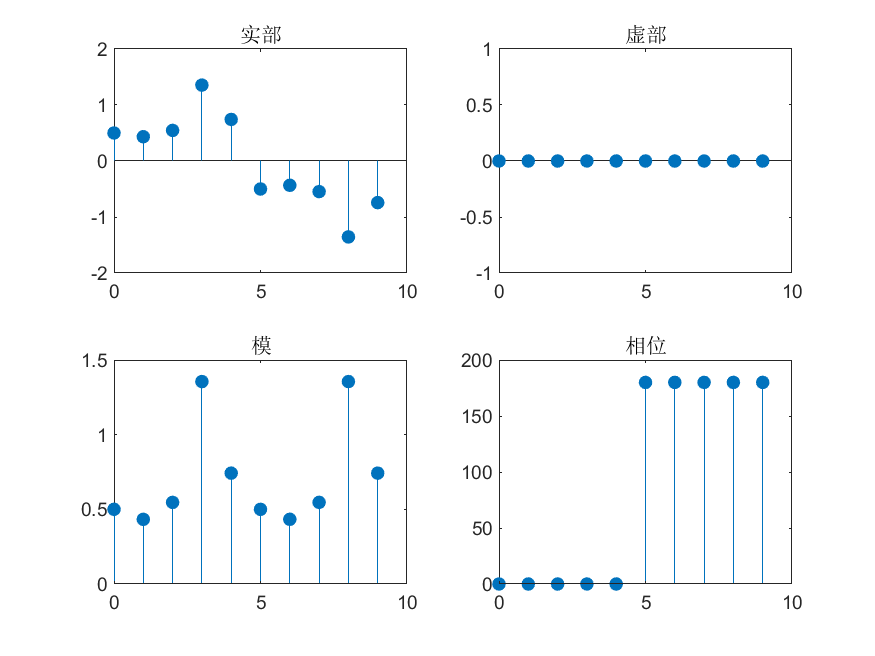
\includegraphics[width=\textwidth]{figure/复合函数序列_phi=90.png}
        \end{minipage}
        \begin{minipage}[t]{0.48\textwidth}
        \centering
        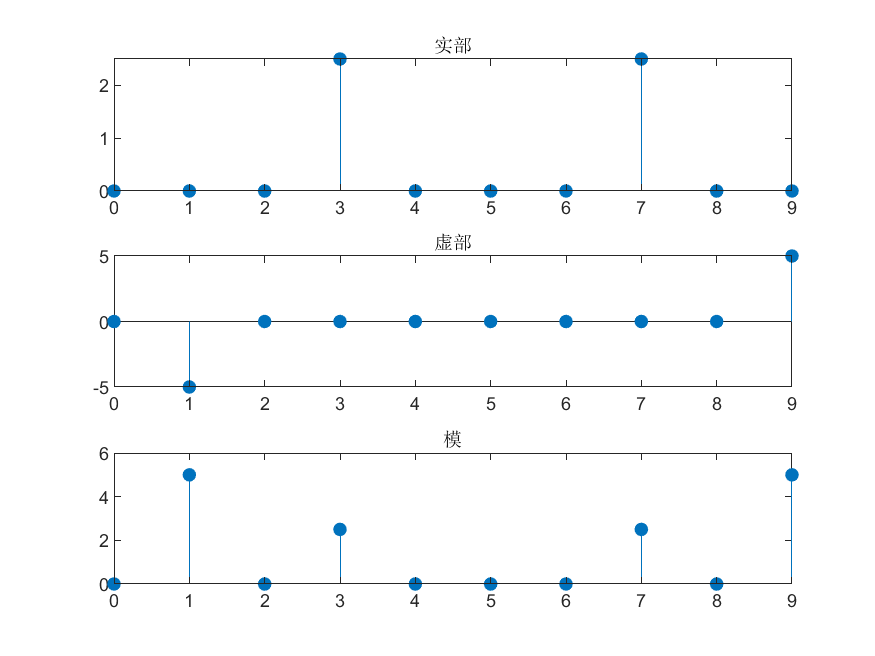
\includegraphics[width=\textwidth]{figure/频谱_复合函数序列_phi=90.png}
        \end{minipage}
    \end{figure}

    \begin{block}{}
        而当 $\phi=90^\circ$ 时,该序列不具备对称性,所以频谱也不具备对称性。但由于复合的序列的频率没变,所以频域谱线仍然出现在 1Hz 与 3Hz 处。
    \end{block}
\end{frame}

\section{实验结论}
\begin{frame}{DFT的物理意义}
    \begin{alertblock}{意义}
        DFT是序列傅里叶变换在$0-2\pi$上的等距采样。
    \end{alertblock}
    \hspace*{\fill} 
    \begin{block}{各个点的意义}
        \begin{enumerate}
            \item X(0):信号直流分量的频谱值
            \item X(1):信号在基频处的幅度和相位
            \item X(N-1):信号在N-1次谐波处的幅度和相位
        \end{enumerate}
    \end{block}
    
\end{frame}

\begin{frame}{DFT的性质}
    \begin{block}{主要性质}
        \begin{enumerate}
            \item \textbf{线性}:如果$x_1(n)$和$x_2(n)$的DFT为$X_1(k)$与$X_2(k)$,则$ax_1(n)+bx_2(n)$的DFT为$aX_1(k)+bX_2(k)$
            \item \textbf{反转定理}:如果$x(n)$的DFT结果为$X(k)$,则$x((-n))_N$的DFT为$X((-k))_N$
            \item \textbf{序列的循环位移}:如果$x(n)$的DFT结果为$X(k)$,则$x((n+m))_N$的DFT为$W_N^{-km}X(k)$
            \item \textbf{卷积性质}:两个序列圆卷积的DFT等于他们分别DFT的结果相乘
            \item \textbf{帕斯瓦尔定理}:$\sum_{n=0}^{N-1}|x(n)|^2 = \frac{1}{N}\sum_{k=0}^{N-1}|X(k)|^2$
        \end{enumerate}
    \end{block}
    
\end{frame}

\end{document}